\documentclass[article,twoside]{combine}

\usepackage[
  paperheight=8.5in,
  paperwidth=5.5in,
  left=10mm,
  right=10mm,
  top=20mm,
  bottom=20mm]{geometry}
\usepackage[utf8]{inputenc}

\usepackage{graphicx}
\usepackage{wrapfig}
\usepackage[bottom]{footmisc}
\usepackage{listings}
\usepackage{enumitem}

\usepackage{wrapfig}
\usepackage{ragged2e}

\usepackage{array}
\usepackage[table]{xcolor}
\usepackage{multirow}
\usepackage{booktabs}
\usepackage{hhline}
\definecolor{palegreen}{rgb}{0.6,0.98,0.6}

\usepackage{amsmath}
\usepackage{amssymb}
\usepackage{multicol}
\usepackage{lipsum}
\usepackage{hyphenat}
\PassOptionsToPackage{hyphens}{url}
\usepackage{url}

\usepackage{rotating}

%\usepackage{xeCJK}

%% support use of straight quotes in code listings
\usepackage[T1]{fontenc}
\usepackage{textcomp}
\usepackage{listings}
\lstset{upquote=true}

%% for shrinking space between lines
\usepackage{setspace}

\newcommand*{\affaddr}[1]{#1} % No op here. Customize it for different styles.
\newcommand*{\affmark}[1][*]{\textsuperscript{#1}}
\newcommand*{\email}[1]{\small{\texttt{#1}}}
\newcommand{\tarot}{\textsc{Tarot}}
\renewcommand*\contentsname{\centering Table of Contents}

\renewcommand{\footnoterule}{%
  \kern -3pt
  \hrule width \textwidth height 0.5pt
  \kern 2pt
}

% remove date
\date{}

\usepackage{titlesec}
\titleformat*{\section}{\large\bfseries}
\titleformat*{\subsection}{\normalsize\bfseries}
\titleformat*{\subsubsection}{\normalsize\bfseries}

\usepackage{biblatex}


\usepackage{algorithm}
\usepackage{algpseudocode}

\begin{document}

\pagestyle{combine} % use the combine page style

\thispagestyle{empty}
\input{title}

\clearpage

% copyright page
\null
\vfill

{\parindent0pt
\textit{The Journal of Computing Sciences in Colleges}
(ISSN 1937-4771 print, 1937-4763 digital) is published at least six times per
year and constitutes the refereed papers of regional conferences sponsored by
the Consortium for Computing Sciences in Colleges.

\vspace{10pt}

Copyright \copyright 2024 by the Consortium for Computing Sciences in Colleges.
Permission to copy without fee all or part of this material is granted provided
that the copies are not made or distributed for direct commercial advantage,
the CCSC copyright notice and the title of the publication and its date appear,
and notice is given that copying is by permission of the Consortium for
Computing Sciences in Colleges.  To copy otherwise, or to republish, requires
a fee and/or specific permission.

}

\clearpage

\tableofcontents % main ToC

\begin{papers}

\coltoctitle{The Consortium for Computing Sciences in Colleges Board of
Directors}
\import{board_directors}

\coltoctitle{CCSC National Partners}
\import{national_partners}

\coltoctitle{Welcome to the \confYear\ CCSC \confName\ Conference}
\import{welcome}

\coltoctitle{Regional Committees --- \confYear\ CCSC \confName\ Region}
\import{regional_committees}

%papers
\coltoctitle{Using Participatory Narrative Inquiry to Explore Cooperative Education in Computing Education}
\coltocauthor{Sebastian Dziallas, University of the Pacific}
\import{paper1.pdf}
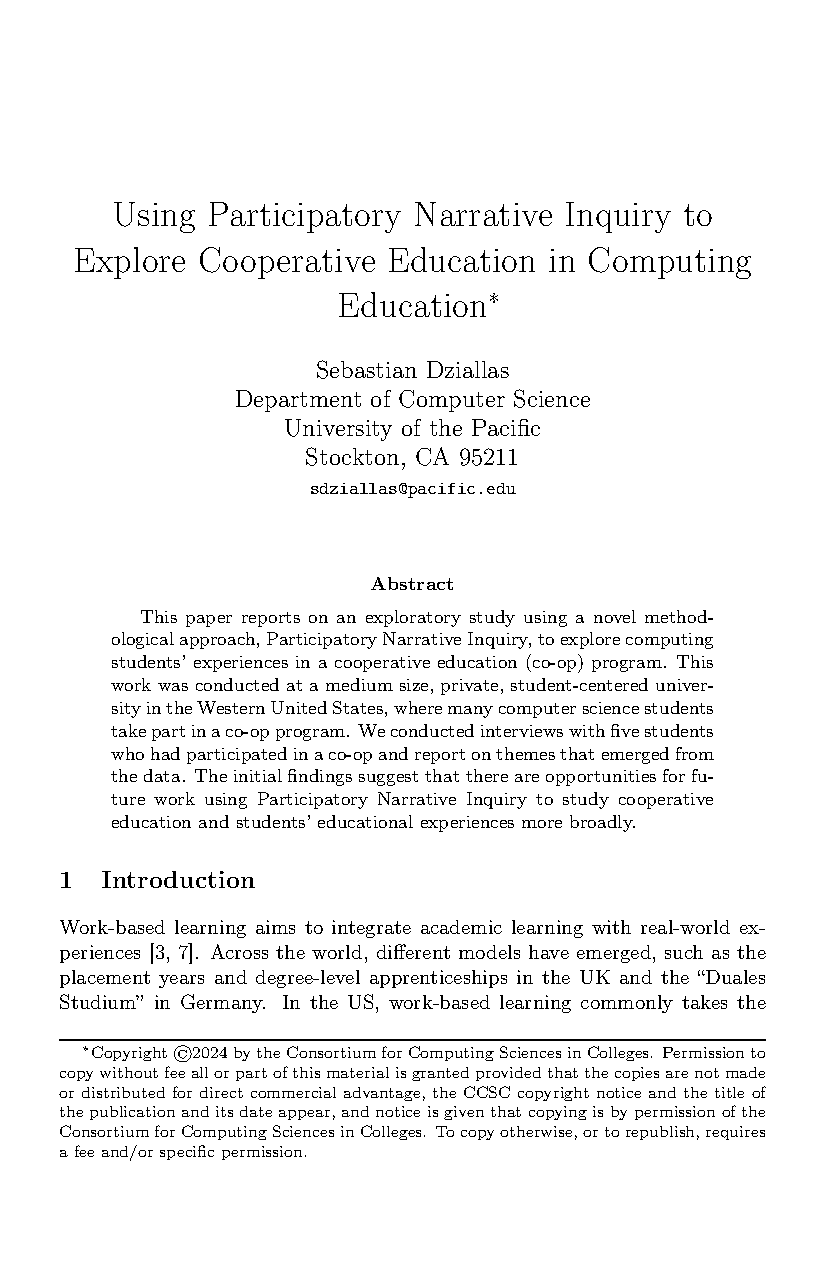
\includepdf[pages=-,pagecommand={\thispagestyle{plain}}]{paper1.pdf} 

\coltoctitle{Investigation of Social Cognitive Factors Affecting Computing Transfer Students}
\coltocauthor{Kay Vargas,  Victor Diaz, Sherrene Bogle, California State Polytechnic University Humboldt,
Shebuti Rayana, SUNY OLD Westbury,
Claire MacDonald, Palvi Aggarwal, University of Texas At El Paso,
Yun Wan, niversity of Houston-Victoria,
Xiwei Wang, Northeastern Illinois University
}
\import{paper2.pdf}
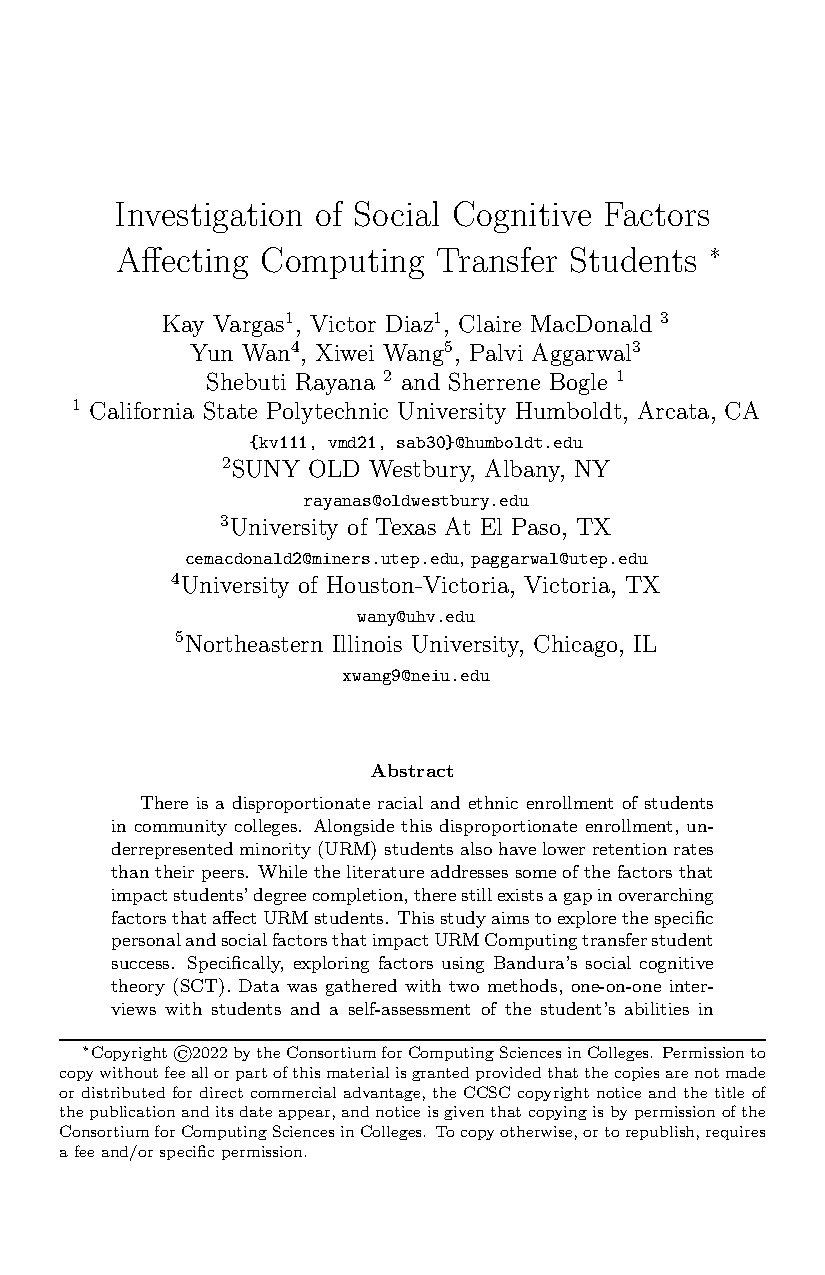
\includepdf[pages=-,pagecommand={\thispagestyle{plain}}]{paper2.pdf} 

\coltoctitle{Rethinking Linear Algebra for Computer Science: Applying Vygotsky’s Theory of Learning}
\coltocauthor{Abbas Attarwala, California State University, Chico}
\import{paper3.pdf}
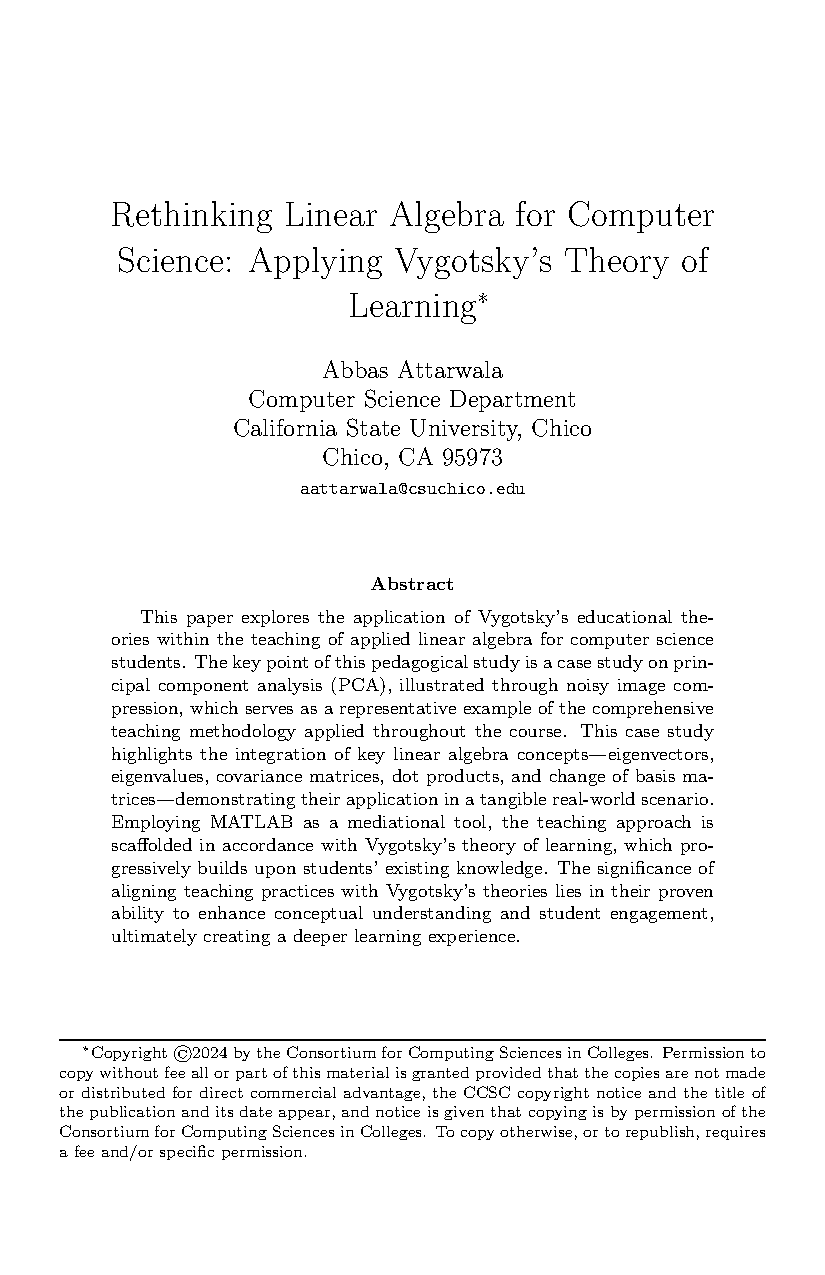
\includepdf[pages=-,pagecommand={\thispagestyle{plain}}]{paper3.pdf} 

\coltoctitle{Reviewers --- \confYear\ CCSC \confName\ Conference}
\import{reviewers}

\end{papers}

\end{document}
